%%%%%%%%%%%%%%%%%%%%%%%%%%%%%%%%%%%%%%%%%%%%%%%%%%%%%%%%%%%%%%%%%%%%%%%%%%%%%%%%%
%% Documenclass 
%%%%%%%%%%%%%%%%%%%%%%%%%%%%%%%%%%%%%%%%%%%%%%%%%%%%%%%%%%%%%%%%%%%%%%%%%%%%%%%%%
\documentclass[a4paper,oneside,titlepage]{report}
%%%%%%%%%%%%%%%%%%%%%%%%%%%%%%%%%%%%%%%%%%%%%%%%%%%%%%%%%%%%%%%%%%%%%%%%%%%%%%%%%
%% Packages
%%%%%%%%%%%%%%%%%%%%%%%%%%%%%%%%%%%%%%%%%%%%%%%%%%%%%%%%%%%%%%%%%%%%%%%%%%%%%%%%%
\usepackage[english]{babel}
\usepackage{kotex}
\usepackage{amsmath}
\usepackage{complexity}
\usepackage[T1]{fontenc}
\usepackage[utf8]{inputenc}
\usepackage[pdftex]{graphicx} %%Graphics in pdfLaTeX
\usepackage{a4wide} %%Smaller margins, more text per page.
\usepackage{longtable} %%For tables that exceed a page width
\usepackage{pdflscape} %%Adds PDF sup­port to the land­scape en­vi­ron­ment of pack­age
\usepackage{caption} %%Pro­vides many ways to cus­tomise the cap­tions in float­ing en­vi­ron­ments like fig­ure and ta­ble
\usepackage{float} %%Im­proves the in­ter­face for defin­ing float­ing ob­jects such as fig­ures and ta­bles
\usepackage[tablegrid,nochapter]{vhistory} %%Vhis­tory sim­pli­fies the cre­ation of a his­tory of ver­sions of a doc­u­ment
\usepackage[nottoc]{tocbibind} %%Au­to­mat­i­cally adds the bib­li­og­ra­phy and/or the in­dex and/or the con­tents, etc., to the Ta­ble of Con­tents list­ing
\usepackage[toc,page]{appendix} %%The ap­pendix pack­age pro­vides var­i­ous ways of for­mat­ting the ti­tles of ap­pen­dices
\usepackage{pdfpages} %%This pack­age sim­pli­fies the in­clu­sion of ex­ter­nal multi-page PDF doc­u­ments in LATEX doc­u­ments
\usepackage[rightcaption]{sidecap} %%De­fines en­vi­ron­ments called SC­fig­ure and SCtable (anal­o­gous to fig­ure and ta­ble) to type­set cap­tions side­ways
\usepackage{cite} %%The pack­age sup­ports com­pressed, sorted lists of nu­mer­i­cal ci­ta­tions, and also deals with var­i­ous punc­tu­a­tion and other is­sues of rep­re­sen­ta­tion, in­clud­ing com­pre­hen­sive man­age­ment of break points
\usepackage[]{acronym} %%This pack­age en­sures that all acronyms used in the text are spelled out in full at least once. It also pro­vides an en­vi­ron­ment to build a list of acronyms used
\usepackage[pdftex,scale={.8,.8}]{geometry} %%The pack­age pro­vides an easy and flex­i­ble user in­ter­face to cus­tomize page lay­out, im­ple­ment­ing auto-cen­ter­ing and auto-bal­anc­ing mech­a­nisms so that the users have only to give the least de­scrip­tion for the page lay­out. For ex­am­ple, if you want to set each mar­gin 2cm with­out header space, what you need is just \usep­a­ck­age[mar­gin=2cm,no­head]{ge­om­e­try}.
\usepackage{layout} %%The pack­age de­fines a com­mand \lay­out, which will show a sum­mary of the lay­out of the cur­rent doc­u­ment
\usepackage{subfigure} %%Pro­vides sup­port for the ma­nip­u­la­tion and ref­er­ence of small or ‘sub’ fig­ures and ta­bles within a sin­gle fig­ure or ta­ble en­vi­ron­ment.
\usepackage[toc]{glossaries} %%The glos­saries pack­age sup­ports acronyms and mul­ti­ple glos­saries, and has pro­vi­sion for op­er­a­tion in sev­eral lan­guages (us­ing the fa­cil­i­ties of ei­ther ba­bel or poly­glos­sia).
\usepackage[left,pagewise,modulo]{lineno} %%Adds line num­bers to se­lected para­graphs with ref­er­ence pos­si­ble through the LATEX \ref and \pageref cross ref­er­ence mech­a­nism
\usepackage[pdftex,colorlinks=false,hidelinks,pdfstartview=FitV]{hyperref}%%The hy­per­ref pack­age is used to han­dle cross-ref­er­enc­ing com­mands in LATEX to pro­duce hy­per­text links in the doc­u­ment. 
\usepackage{metainfo}
\usepackage[pagestyles,raggedright]{titlesec}
\usepackage{etoolbox}
\usepackage{%
	array, %%An ex­tended im­ple­men­ta­tion of the ar­ray and tab­u­lar en­vi­ron­ments which ex­tends the op­tions for col­umn for­mats, and pro­vides "pro­grammable" for­mat spec­i­fi­ca­tions
	booktabs, %%The pack­age en­hances the qual­ity of ta­bles in LATEX, pro­vid­ing ex­tra com­mands as well as be­hind-the-scenes op­ti­mi­sa­tion
	dcolumn, %%
	rotating,
	shortvrb,
	units,
	url,
	lastpage,
	longtable,
	lscape,
	qtree,
	skmath,	
}
%%%%%%%%%%%%%%%%%%%%%%%%%%%%%%%%%%%%%%%%%%%%%%%%%%%%%%%%%%%%%%%%%%%%%%%%%%%%%%%%%
%% Java --> latex 
%%%%%%%%%%%%%%%%%%%%%%%%%%%%%%%%%%%%%%%%%%%%%%%%%%%%%%%%%%%%%%%%%%%%%%%%%%%%%%%%%
\usepackage{listings}
\usepackage{color}
\definecolor{pblue}{rgb}{0.13,0.13,1}
\definecolor{pgreen}{rgb}{0,0.5,0}
\definecolor{pred}{rgb}{0.9,0,0}
\definecolor{pgrey}{rgb}{0.46,0.45,0.48}
\usepackage{inconsolata}
%%Listing style for java.
\definecolor{dkgreen}{rgb}{0,0.6,0}
\definecolor{gray}{rgb}{0.5,0.5,0.5}
\definecolor{mauve}{rgb}{0.58,0,0.82}
\lstset{frame=tb,
	language=Java,
	aboveskip=3mm,
	belowskip=3mm,
	showstringspaces=false,
	columns=flexible,
	basicstyle={\small\ttfamily},
	numbers=left,
	numberstyle=\tiny\color{gray},
	keywordstyle=\color{blue},
	commentstyle=\color{dkgreen},
	stringstyle=\color{mauve},
	breaklines=true,
	breakatwhitespace=true,
	tabsize=3
}

%%%%%%%%%%%%%%%%%%%%%%%%%%%%%%%%%%%%%%%%%%%%%%%%%%%%%%%%%%%%%%%%%%%%%%%%%%%%%%%%%
\setlength{\parindent}{0pt}
\setlength{\parskip}{.5\baselineskip}
%%%%%%%%%%%%%%%%%%%%%%%%%%%%%%%%%%%%%%%%%%%%%%%%%%%%%%%%%%%%%%%%%%%%%%%%%%%%%%%%%
%% Inserting the metadata
%%%%%%%%%%%%%%%%%%%%%%%%%%%%%%%%%%%%%%%%%%%%%%%%%%%%%%%%%%%%%%%%%%%%%%%%%%%%%%%%%
% % Metadaten des Dokumentes

\def\Company{Consultancy}
\def\Institute{\textit{Fontys Hogeschool Techniek en Logistiek, Venlo}}
\def\Course{\textit{Software Engineering}}
\def\Module{\textit{ }}
\def\Docent{\textit{}}
\def\Assistant{\textit{}}

\def\BoldTitle{Software Requirements Specification}

\def\Subtitle{for \\ High school scheduling system \\}
\def\Authors{Prepared by:\\\\ XYZ (2434954) \\ ABC (123897) } 
\def\Shortname{A.Sandu}


\title{\textbf{\BoldTitle}\\\Subtitle}
\author{\Authors \\ \\ \\ \Institute\\ \Course\\ \Module\\ \Docent\\ \Assistant}
\date{Venlo, 25. September 2016}

%%%%%%%%%%%%%%%%%%%%%%%%%%%%%%%%%%%%%%%%%%%%%%%%%%%%%%%%%%%%%%%%%%%%%%%%%%%%%%%%%
%% Creation of pdf information
%%%%%%%%%%%%%%%%%%%%%%%%%%%%%%%%%%%%%%%%%%%%%%%%%%%%%%%%%%%%%%%%%%%%%%%%%%%%%%%%%
\hypersetup{pdfinfo={
		Title={Title},
		Author={TR},
		Subject={Report}
	}}
%%%%%%%%%%%%%%%%%%%%%%%%%%%%%%%%%%%%%%%%%%%%%%%%%%%%%%%%%%%%%%%%%%%%%%%%%%%%%%%%%
%% Creating the frontpage
%%%%%%%%%%%%%%%%%%%%%%%%%%%%%%%%%%%%%%%%%%%%%%%%%%%%%%%%%%%%%%%%%%%%%%%%%%%%%%%%%
\AtBeginDocument{
	\maketitle
	\thispagestyle{empty}
}

%%%%%%%%%%%%%%%%%%%%%%%%%%%%%%%%%%%%%%%%%%%%%%%%%%%%%%%%%%%%%%%%%%%%%%%%%%%%%%%%%
%% Creation of the header
%%%%%%%%%%%%%%%%%%%%%%%%%%%%%%%%%%%%%%%%%%%%%%%%%%%%%%%%%%%%%%%%%%%%%%%%%%%%%%%%%
\patchcmd{\chapter}{plain}{short}{}{} %$ <-- the header on chapter 1
%%%%%%%%%%%%%%%%%%%%%%%%%%%%%%%%%%%%%%%%%%%%%%%%%%%%%%%%%%%%%%%%%%%%%%%%%%%%%%%%%
%% Creation of page-styles
%%%%%%%%%%%%%%%%%%%%%%%%%%%%%%%%%%%%%%%%%%%%%%%%%%%%%%%%%%%%%%%%%%%%%%%%%%%%%%%%%
\newpagestyle{long}{%
	\sethead[\thepage][][\chaptername\ \thechapter:\ \chaptertitle]{\chaptername\ \thechapter:\ \chaptertitle}{}{\thepage}
	\headrule
}

\newpagestyle{short}{%
	\sethead[\thepage][][]{}{}{\thepage}
	\headrule
}
%%%%%%%%%%%%%%%%%%%%%%%%%%%%%%%%%%%%%%%%%%%%%%%%%%%%%%%%%%%%%%%%%%%%%%%%%%%%%%%%%
%% DOCUMENT
%%%%%%%%%%%%%%%%%%%%%%%%%%%%%%%%%%%%%%%%%%%%%%%%%%%%%%%%%%%%%%%%%%%%%%%%%%%%%%%%%
\begin{document}

\pagenumbering{roman}
\DeclareGraphicsExtensions{.pdf,.jpg,.png}
\pagestyle{short}



\newpage
%%%%%%%%%%%%%%%%%%%%%%%%%%%%%%%%%%%%%%%%%%%%%%%%%%%%%%%%%%%%%%%%%%%%%%%%%%%%%%%%%
%% Table of contents
%%%%%%%%%%%%%%%%%%%%%%%%%%%%%%%%%%%%%%%%%%%%%%%%%%%%%%%%%%%%%%%%%%%%%%%%%%%%%%%%%
 \tableofcontents % Inhaltsverzeichnis



\pagestyle{long}




%%%%%%%%%%%%%%%%%%%%%%%%%%%%%%%%%%%%%%%%%%%%%%%%%%%%%%%%%%%%%%%%%%%%%%%%%%%%%%%%%
%% Version table insertion
%%%%%%%%%%%%%%%%%%%%%%%%%%%%%%%%%%%%%%%%%%%%%%%%%%%%%%%%%%%%%%%%%%%%%%%%%%%%%%%%%
%% Versionstabelle.

\chapter*{Revision History}
\addcontentsline{toc}{chapter}{Revision History}
\begin{versionhistory}
	\vhEntry{1.0}{25.09.2016}{A.Sandu}{Chapter 1 - Introduction}
    \vhEntry{2.0}{10.12.2015}{}{Explaining different sortings}
    \vhEntry{3.0}{05.01.2016}{}{Kleine Änderungen}
    \vhEntry{4.0}{10.01.2016}{}{Finale Version}


\end{versionhistory}
\pagenumbering{arabic}
%%%%%%%%%%%%%%%%%%%%%%%%%%%%%%%%%%%%%%%%%%%%%%%%%%%%%%%%%%%%%%%%%%%%%%%%%%%%%%%%%
%% Inserting all the content
%%%%%%%%%%%%%%%%%%%%%%%%%%%%%%%%%%%%%%%%%%%%%%%%%%%%%%%%%%%%%%%%%%%%%%%%%%%%%%%%%
\chapter{Introduction}
\label{ch:intro}

\section{Purpose}
The purpose of this document is to define the objectives and scope of the \textbf{[Project Name]}. This ensures that all stakeholders have a clear understanding of the project and agree on what will be delivered.


\section{Product Scope}
This section outlines the boundaries of the product, including the functionalities and features to be delivered. It also specifies any constraints and limitations, ensuring that expectations are aligned with project deliverables.

\section{Definitions, Acronyms, and Abbreviations}
\begin{itemize}
    \item \textbf{API}: Application Programming Interface
    \item \textbf{GUI}: Graphical User Interface
    \item \textbf{SDK}: Software Development Kit
\end{itemize}
Definitions and abbreviations relevant to this document are provided to ensure clarity and avoid any ambiguity.

\section{References}
This section lists references to other relevant documents or materials that were used in the creation of this document:
\begin{itemize}
    \item ISO/IEC 12207:2008 - Systems and software engineering — Software life cycle processes.
    \item Feasibility Study Report, Version 1.0.
\end{itemize}

\section{Overview}
This document is organized as follows:
\begin{itemize}
    \item Section~\ref{ch:intro} introduces the project, providing details about its purpose, scope, and relevant definitions.
    \item Section~2 outlines the technical specifications and requirements.
    \item Section~3 describes the design and implementation approach.
\end{itemize}


\chapter{Overall Description}
\label{ch:overall_desc}

\section{Product Perspective}
This section provides a high-level view of the product, its background, and its positioning in the market.

\subsection{Market Status}
The current market landscape is reviewed to highlight existing solutions and gaps. This analysis provides the context for the product's development and its unique value proposition.

\subsection{Overall Structure}
The overall structure of the product is described, including its components and their interactions. This section provides a conceptual understanding of how the product operates.

\section{Product Functions}
The core functionalities of the product are outlined. Each function is briefly described to provide an understanding of the features that the product offers to its users.

\section{User Classes and Characteristics}
This section identifies the different types of users and their specific characteristics.

\subsection{User}
The end-user category includes individuals who interact with the product to achieve their objectives. Their roles, goals, and skill levels are described here.

\subsection{System Manager}
System managers are responsible for the maintenance and administration of the product. Their roles include configuration, monitoring, and troubleshooting.

\section{Operating Environment}
The operating environment outlines the conditions under which the product will function.

\subsection{Hardware}
The hardware requirements, including specifications for servers, devices, and peripherals, are listed here.

\subsection{Software}
The software environment, including operating systems, third-party applications, and dependencies required to run the product, is described.

\section{Implementation Constraints}
Any constraints that may impact the implementation of the product are identified. These can include technical limitations, regulatory requirements, or organizational policies.

\section{User Documentation}
This section outlines the documentation that will be provided to users, including manuals, tutorials, and online help resources.

\section{Assumptions and Dependencies}
The assumptions made during the product development and any dependencies on external systems, services, or technologies are detailed here.

\chapter{System Requirements}
\label{ch:system_requirements}

\section{External Interface Requirements}
This section describes the interfaces between the system and its external entities.

\subsection{User Interfaces}
The user interface should be intuitive and user-friendly. Below is a mockup example:

\begin{figure}[h]
    \centering
    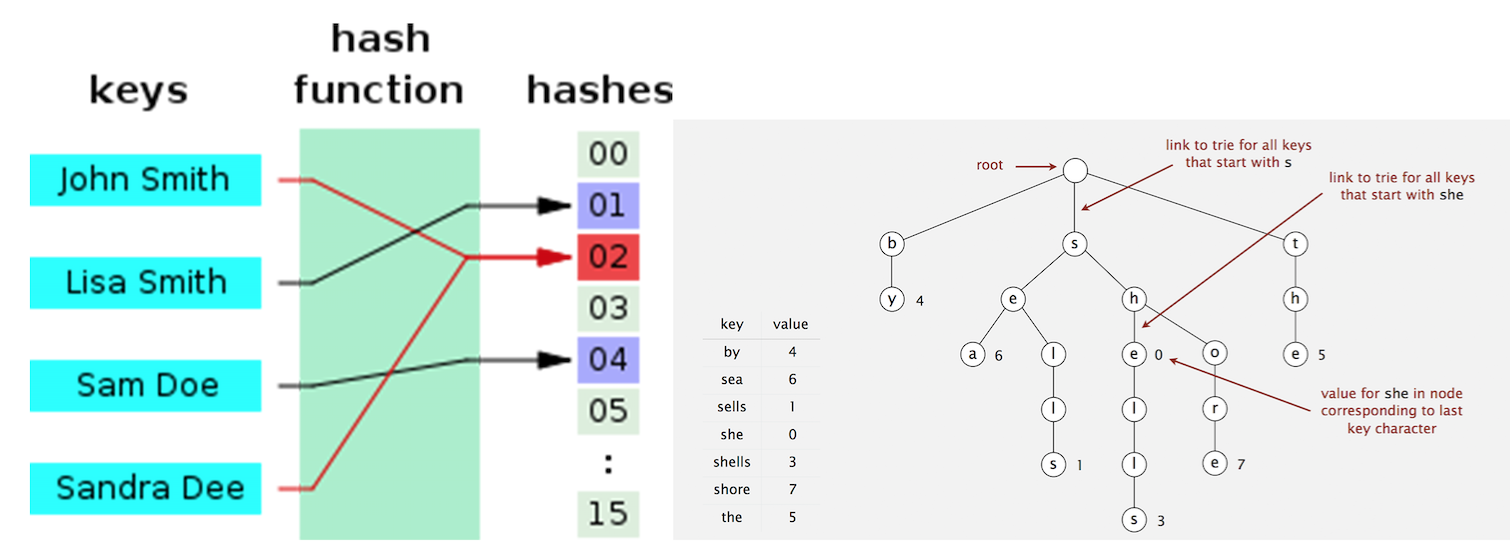
\includegraphics[width=0.8\textwidth]{images/hashing.png}
    \caption{Example User Interface Mockup}
    \label{fig:ui_mockup}
\end{figure}

\subsection{Hardware Interfaces}
The system interfaces with various hardware components, such as sensors and servers. Table~\ref{tab:hardware_interfaces} lists the hardware requirements.

\begin{table}[h]
    \centering
    \begin{tabular}{|l|l|l|}
        \hline
        \textbf{Hardware Component} & \textbf{Specification} & \textbf{Purpose} \\ \hline
        Sensor A & 1080p Resolution & Capturing data \\ \hline
        Server X & 16-Core CPU, 64GB RAM & Data processing \\ \hline
        Display Monitor & 1920x1080 Resolution & User interface \\ \hline
    \end{tabular}
    \caption{Hardware Interfaces}
    \label{tab:hardware_interfaces}
\end{table}

\subsection{Software Interfaces}
The required software interfaces include third-party libraries, APIs, and other software systems that interact with the product. Figure~\ref{fig:software_architecture} provides an overview of the software architecture.

\begin{figure}[h]
    \centering
    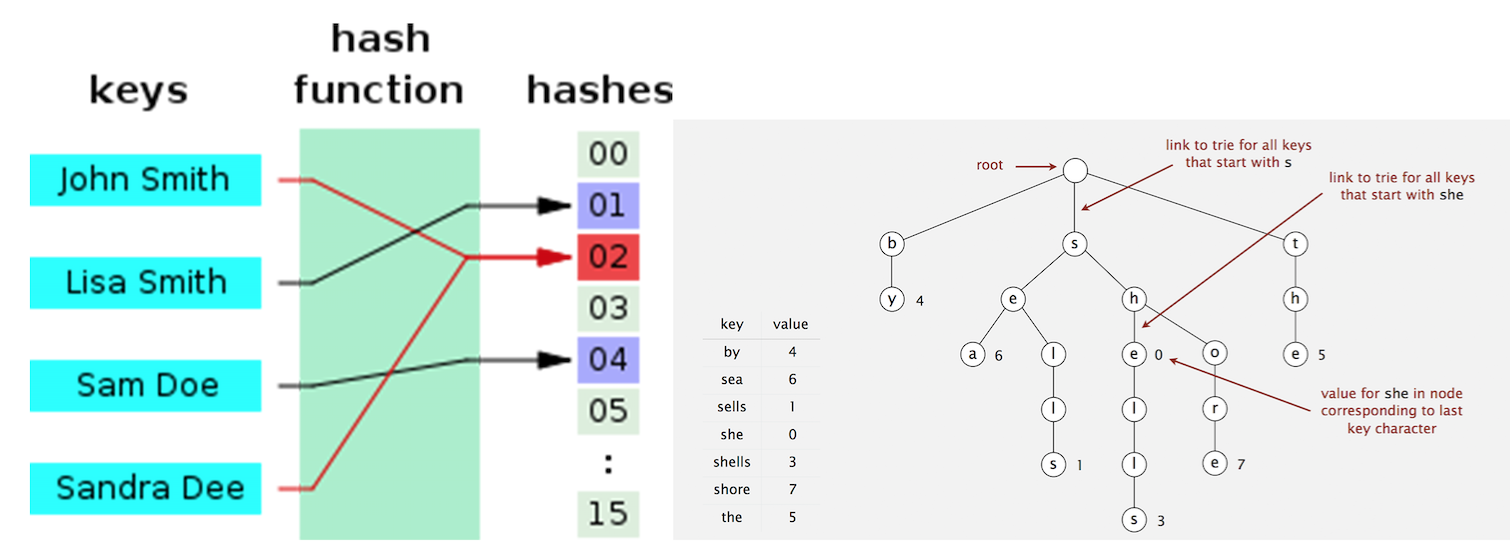
\includegraphics[width=0.8\textwidth]{images/hashing.png}
    \caption{Software Architecture Diagram}
    \label{fig:software_architecture}
\end{figure}

\subsection{Communication Interfaces}
The system will utilize HTTP and WebSocket protocols for communication between components. Table~\ref{tab:communication_interfaces} lists the communication protocols.

\begin{table}[h]
    \centering
    \begin{tabular}{|l|l|}
        \hline
        \textbf{Protocol} & \textbf{Usage} \\ \hline
        HTTP & Standard API communication \\ \hline
        WebSocket & Real-time updates \\ \hline
    \end{tabular}
    \caption{Communication Interfaces}
    \label{tab:communication_interfaces}
\end{table}

\section{Functional Requirements}
The functional requirements specify the system's behavior.

\subsection{Use Case}
Below is an example use case for user login:

\begin{table}[h]
    \centering
    \begin{tabular}{|l|l|}
        \hline
        \textbf{Use Case ID} & UC001 \\ \hline
        \textbf{Use Case Name} & User Login \\ \hline
        \textbf{Description} & Allows users to log into the system \\ \hline
        \textbf{Actors} & End User \\ \hline
        \textbf{Preconditions} & User has valid credentials \\ \hline
        \textbf{Postconditions} & User is logged in \\ \hline
    \end{tabular}
    \caption{Use Case Example}
    \label{tab:use_case}
\end{table}

\subsection{Use Case Diagram}
An example use case diagram is shown in Figure~\ref{fig:use_case_diagram}.

\begin{figure}[h]
    \centering
    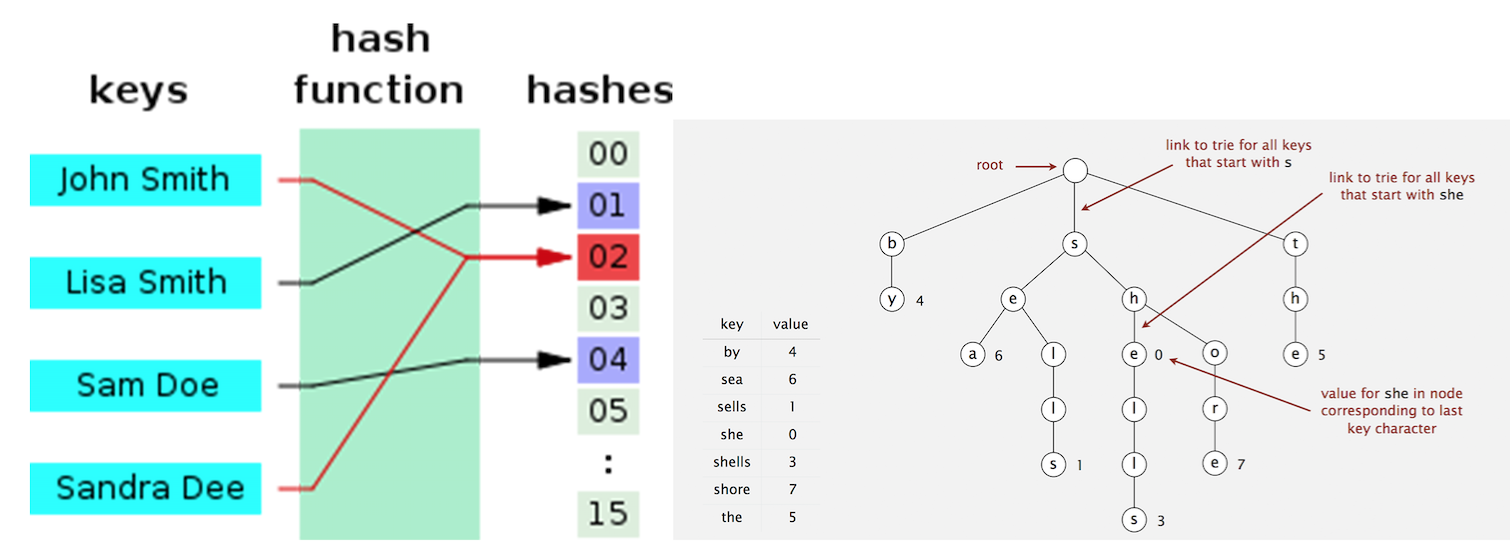
\includegraphics[width=0.7\textwidth]{images/hashing.png}
    \caption{Use Case Diagram}
    \label{fig:use_case_diagram}
\end{figure}

\subsection{Data Dictionary}
The data dictionary defines key data elements in the system. Table~\ref{tab:data_dictionary} provides an example.

\begin{table}[h]
    \centering
    \begin{tabular}{|l|l|l|}
        \hline
        \textbf{Field Name} & \textbf{Data Type} & \textbf{Description} \\ \hline
        UserID & Integer & Unique identifier for each user \\ \hline
        Username & String & User's login name \\ \hline
        PasswordHash & String & Encrypted user password \\ \hline
    \end{tabular}
    \caption{Data Dictionary Example}
    \label{tab:data_dictionary}
\end{table}

\section{Non-functional Requirements}

\subsection{Product Requirements}
The system must meet performance benchmarks. Table~\ref{tab:performance_requirements} highlights key metrics.

\begin{table}[h]
    \centering
    \begin{tabular}{|l|l|}
        \hline
        \textbf{Metric} & \textbf{Requirement} \\ \hline
        Response Time & Less than 200ms for 95\% of requests \\ \hline
        Uptime & 99.9\% availability \\ \hline
        Scalability & Support up to 10,000 concurrent users \\ \hline
    \end{tabular}
    \caption{Performance Requirements}
    \label{tab:performance_requirements}
\end{table}

\section{API Specifications}
Figure~\ref{fig:api_interaction} illustrates the interaction between different APIs.

\begin{figure}[h]
    \centering
    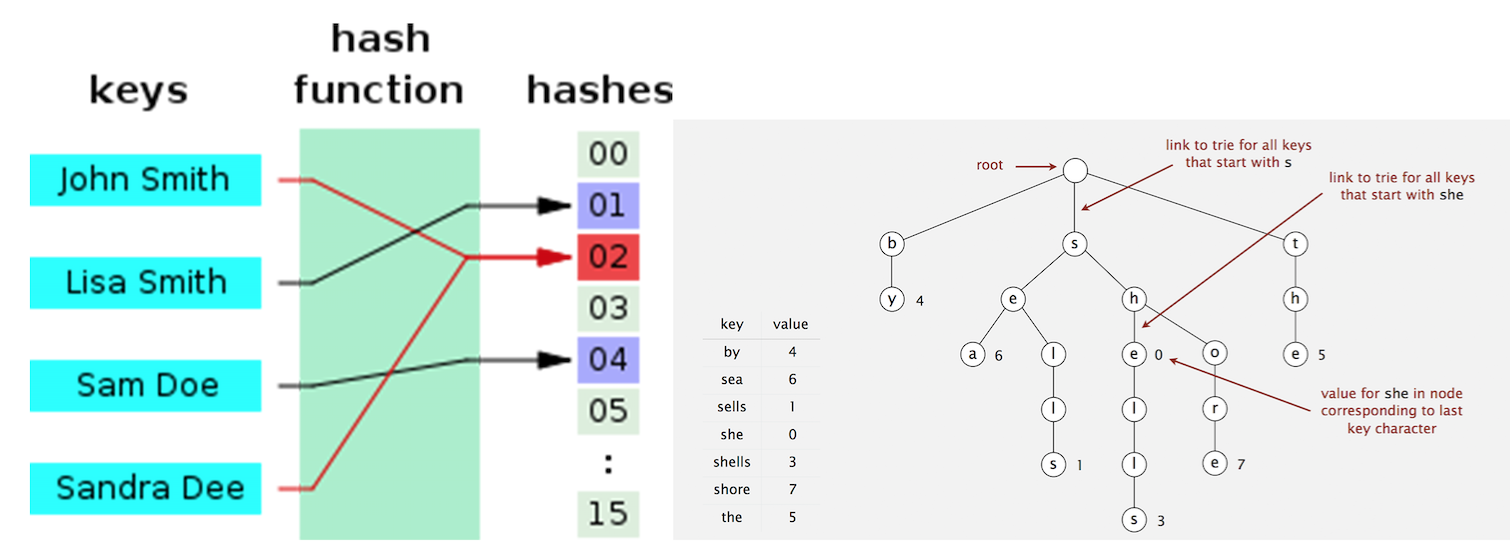
\includegraphics[width=0.9\textwidth]{images/hashing.png}
    \caption{API Interaction Diagram}
    \label{fig:api_interaction}
\end{figure}

\section{Main Chain Architecture}
The main chain architecture, as illustrated in Figure~\ref{fig:main_chain}, shows the core workflow.

\begin{figure}[h]
    \centering
    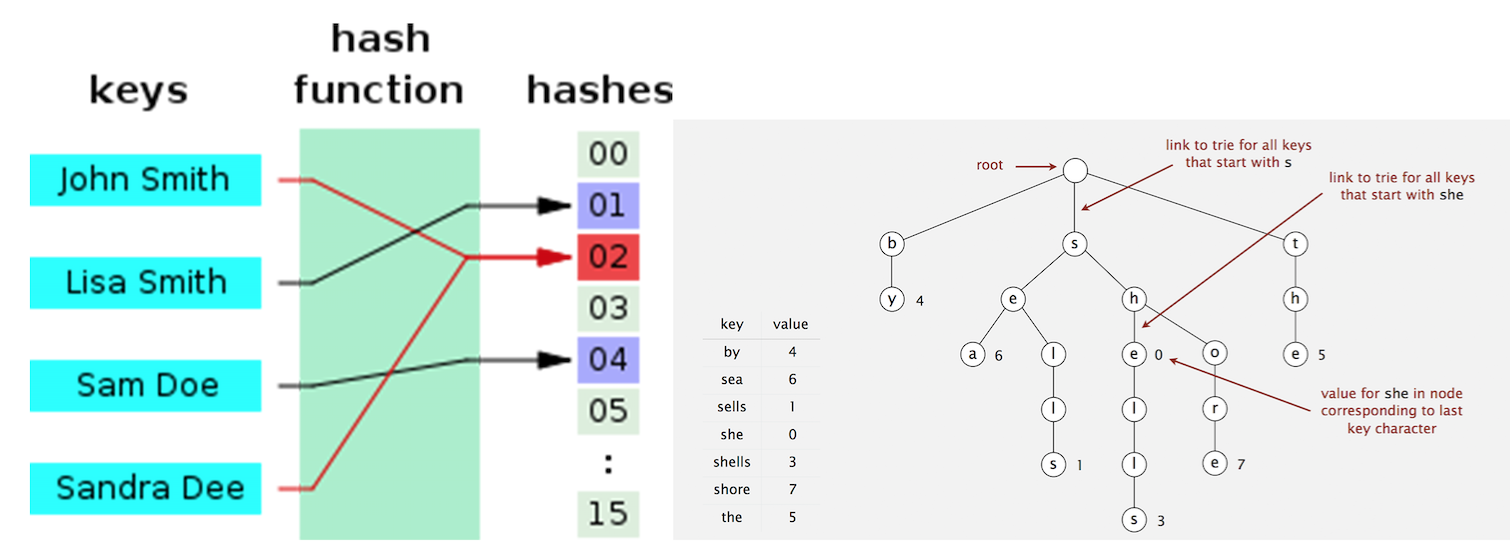
\includegraphics[width=0.8\textwidth]{images/hashing.png}
    \caption{Main Chain Architecture}
    \label{fig:main_chain}
\end{figure}

\section{Database Architecture}
The database schema is presented in Figure~\ref{fig:database_schema}.

\begin{figure}[h]
    \centering
    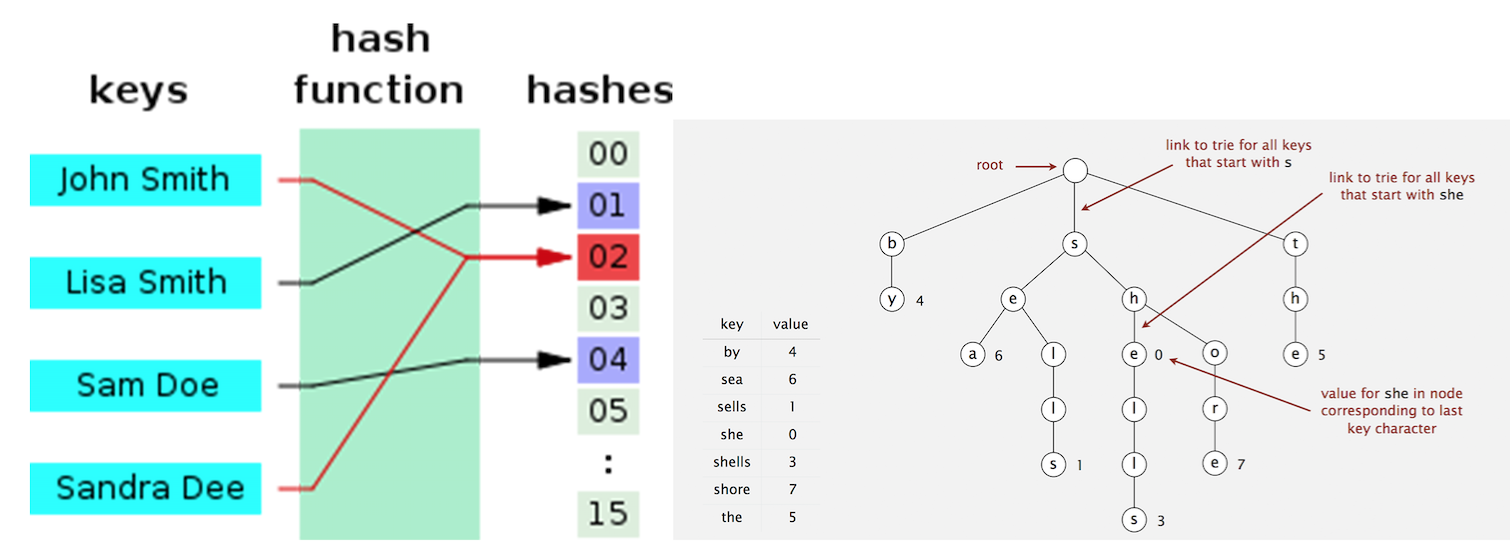
\includegraphics[width=0.8\textwidth]{images/hashing.png}
    \caption{Database Schema}
    \label{fig:database_schema}
\end{figure}

\section{System Evolution}
\subsection{Limitation and Assumption}
The system assumes constant network availability, which may limit usage in offline environments.

\subsection{Anticipated Changes}
Future updates will include machine learning capabilities for enhanced predictions.

\chapter{Supporting Information}
\label{ch:supporting_information}

\section{Software Requirements}
This section lists the software requirements necessary for the system to function correctly. Table~\ref{tab:software_requirements} provides the details.

\begin{table}[h]
    \centering
    \begin{tabular}{|l|l|l|}
        \hline
        \textbf{Software} & \textbf{Requirement} & \textbf{Specification} \\ \hline
        Operating System & Linux/Windows & Ubuntu 20.04 or later, Windows 10 \\ \hline
        Database & MySQL & Version 8.0 or higher \\ \hline
        Web Server & Nginx/Apache & Nginx 1.18+ or Apache 2.4+ \\ \hline
        Programming Language & Python & Version 3.8 or higher \\ \hline
        Framework & Django & Version 4.0 or higher \\ \hline
        Frontend Framework & React & Version 18.0 or higher \\ \hline
    \end{tabular}
    \caption{Software Requirements}
    \label{tab:software_requirements}
\end{table}

\section{Additional Resources}
This section provides information about additional resources that may be required for the project.

\subsection{Documentation}
The system includes comprehensive documentation:
\begin{itemize}
    \item User Manual: Instructions for end users.
    \item Developer Guide: Technical details for developers.
    \item API Documentation: Specifications for API usage.
\end{itemize}

\subsection{External Libraries and Tools}
The following libraries and tools are recommended:
\begin{itemize}
    \item \textbf{NumPy}: For numerical operations.
    \item \textbf{Pandas}: For data manipulation.
    \item \textbf{Matplotlib}: For visualizations.
    \item \textbf{Docker}: For containerization.
\end{itemize}

\section{System Compatibility}
The system is designed to be compatible with various hardware and software configurations. Compatibility details include:
\begin{itemize}
    \item \textbf{Browsers}: Chrome, Firefox, Edge.
    \item \textbf{Devices}: Desktop, tablet, mobile.
\end{itemize}

\section{Reference Materials}
For further information, the following materials are referenced:
\begin{itemize}
    \item Project Feasibility Study
    \item Industry Standards Documentation
    \item Third-Party Library Manuals
\end{itemize}




\begin{appendices}
\chapter{Glossary}
\chapter{Analysis Models}
\chapter{To be detrmined List}
\end{appendices}





%%%%%%%%%%%%%%%%%%%%%%%%%%%%%%%%%%%%%%%%%%%%%%%%%%%%%%%%%%%%%%%%%%%%%%%%%%%%%%%%%
%% Source defintions
%%%%%%%%%%%%%%%%%%%%%%%%%%%%%%%%%%%%%%%%%%%%%%%%%%%%%%%%%%%%%%%%%%%%%%%%%%%%%%%%%
% When no use outcomment
%\bibliographystyle{alpha}

\renewcommand\bibname{References}
\bibliography{base/sources}


%%%%%%%%%%%%%%%%%%%%%%%%%%%%%%%%%%%%%%%%%%%%%%%%%%%%%%%%%%%%%%%%%%%%%%%%%%%%%%%%%
%% Inserting the appendix
%%%%%%%%%%%%%%%%%%%%%%%%%%%%%%%%%%%%%%%%%%%%%%%%%%%%%%%%%%%%%%%%%%%%%%%%%%%%%%%%%
% When no use outcomment
%\newpage
\appendix 
% Adds appendix as chapter to toc
\addcontentsline{toc}{chapter}{Appendix}


\chapter{First}


\chapter{Second}


\end{document}*/***********************************************************************8	
